\documentclass{article}
\usepackage{color}
\usepackage{tikz}

% Tikz settings optimized for causal graphs.
% Just copy-paste this part
\usetikzlibrary{shapes,decorations,arrows,calc,arrows.meta,fit,positioning}
\tikzset{
    -Latex,auto,node distance =1 cm and 1 cm,semithick,
    state/.style ={ellipse, draw, minimum width = 0.7 cm},
    point/.style = {circle, draw, inner sep=0.04cm,fill,node contents={}},
    bidirected/.style={Latex-Latex,dashed},
    el/.style = {inner sep=2pt, align=left, sloped}
}

\begin{document}
\section{Data Prep, EDA, and Theory development}
\subsection{Varaible Selection \& Explanation}
\indent For the purpose of analyzing the determinats of house (sales) prices in the US a theory was developed based on combining two common valuation strategies in real-estate; "vergleichswert verfahren, sachwert verfahren".

\indent Based on the theory, four categories of regressors were identified in the data, promising to best represent the population regression equation. 
\begin{itemize}
  \item Size related quantities (House size, lot size); garage
  \item District and Neighborhood dependent variables; Zoning
  \item type of housing (one family home, apartment, etc)
  \item Quality and condition of the house; including time since remodeling
\end{itemize}

To this end, this reasearch assignemnt draws data from an apprisal project conducted by... in the Ames district, Iowa (USA) (CITE DATA SOURCE HERE!!!). Corresponding to the aforementioned data categories, the following variables were selected to be used in varying degrees in the model. It may be noted, that due to the data being limited to a city in the midwest of the USA, the generalization resulting from this research may only extend to similar cities. However, due to the data originating from one district alone results in the comparability of the sale instances recorded in the data; meaning that stark contrasts in sales prices may be less due to the simple fact that one sale may have been made in Iowa and the other in New York, which naturally yields higher prices.

To start, a total of 1,460 house sales were recorded between 2006 and 2010 for the district of Ames, Iowa (USA). The dependent varibale was identified to be SalePrice. As can be observed in Table 1, the mean sale price of a house was \$180,921.20 (SD = 79,442.50). Combined with the range [34,900, 755,000] a positive skewness was to be expected (skew = 1.881), considering that the outcome variable is a of financial nature.

\indent Following, the first category of data pertains to size related dimensions of the property sold. More specifically, the total living area (tot\_living\_area)\footnote{defined as summing above- and below- ground or base living.} displays a mean of 2,572.89 square feet (SD = 823.598) in addition to a large reange of values[334, 11,752]; suggesting that the sales were conducted in neighborhoods (Neighborhood) included range from urban to (partially) rural. To this end, the second data category encompasses the zoning classification (MSZoning) which identifies neighborhoods and the correpsonding sales as rural or not. Neighborhood consisists of 25 distinctions and zoning of eight categories\footnote{only 5 categories actually contain data.}, which will be adjusted to three categories to decrease the complexity of the data analysis (see Appendix for a contignecy table). Additionally, the number of bedrooms above ground level (mean = 2.866, SD = 0.816) (BedroomAbvGr) and the number of bathrooms (mean = 1.990, SD = 0.732) are included (tot\_bathrooms)\footnote{The correlation betwen house size and number of bedrooms and bathrooms will be addressed later}. 
\indent Moreover, the third class of data was selected to balance size and neighborhood related associations by consideringh building type (BldgType), which consists of five categories. Interestingly, the majority of sold homes were one-family homes (n = 1220); this variable was adjusted to reduce the complexity of the data analysis and remove confusion about the definition of building type.
\indent The fourth category contains quality and condition related variables. Both variables are on a discrete  scale from one to ten. Quality displays values for each quality rating (mean = 6.099, SD = 1.383), while the condition ranges from one to nine (mean = 5.575, SD = 1.113).
 

% Table created by stargazer v.5.2.3 by Marek Hlavac, Social Policy Institute. E-mail: marek.hlavac at gmail.com
% Date and time: Fri, Sep 09, 2022 - 12:53:46
\begin{table}[!htbp] \centering 
  \caption{Descriptive Statistics} 
  \label{} 
\begin{tabular}{@{\extracolsep{5pt}}lccccc} 
\\[-1.8ex]\hline 
\hline \\[-1.8ex] 
Statistic & \multicolumn{1}{c}{N} & \multicolumn{1}{c}{Mean} & \multicolumn{1}{c}{St. Dev.} & \multicolumn{1}{c}{Min} & \multicolumn{1}{c}{Max} \\ 
\hline \\[-1.8ex] 
SalePrice & 1,460 & 180,921.200 & 79,442.500 & 34,900 & 755,000 \\ 
YearBuilt & 1,460 & 1,971.268 & 30.203 & 1,872 & 2,010 \\ 
YearRemodAdd & 1,460 & 1,984.866 & 20.645 & 1,950 & 2,010 \\ 
LotArea & 1,460 & 10,516.830 & 9,981.265 & 1,300 & 215,245 \\ 
GrLivArea & 1,460 & 1,515.464 & 525.480 & 334 & 5,642 \\ 
TotalBsmtSF & 1,460 & 1,057.429 & 438.705 & 0 & 6,110 \\ 
BedroomAbvGr & 1,460 & 2.866 & 0.816 & 0 & 8 \\ 
BsmtFullBath & 1,460 & 0.425 & 0.519 & 0 & 3 \\ 
FullBath & 1,460 & 1.565 & 0.551 & 0 & 3 \\ 
GarageCars & 1,460 & 1.767 & 0.747 & 0 & 4 \\ 
OverallQual & 1,460 & 6.099 & 1.383 & 1 & 10 \\ 
OverallCond & 1,460 & 5.575 & 1.113 & 1 & 9 \\ 
tot\_living\_area & 1,460 & 2,572.893 & 823.598 & 334 & 11,752 \\ 
tot\_bathrooms & 1,460 & 1.990 & 0.732 & 0 & 6 \\ 
\hline \\[-1.8ex] 
\end{tabular} 
\end{table} 


It is notable that upon selecting the aforementioned variables, no preprossessing in the form of imputation or data deletion had to be applied. However, in order to decrease the complecity of the interaction term, the variable MSZoning was binned into (rural, mixed rural, and urban) based on the corresponding zoning categories\footnote{$https://www.kaggle.com/competitions/home-data-for-ml-course/data$}.


\subsection{Exploratory Data Analysis}\footnote{The theory underlying the choice of the variables will be further elaborated upon in Section 2}
A scatter plot matrix is provided in the appendix for the numeric variables. The EDA shows the four data categories with respect to the sale price of the property. Thus, the plots represented, inter alia, drove the development of the hypothesis down the line in combination with the aforementioned valuation strategies. 



first analysis:
Size of living area to sales price with respect to building type

Second analysis
total rooms and sales price with respect to size zoning

Third analysis
quality and condition to sales price



\section{Theoretical model and OLS assumptions}




\begin{center}
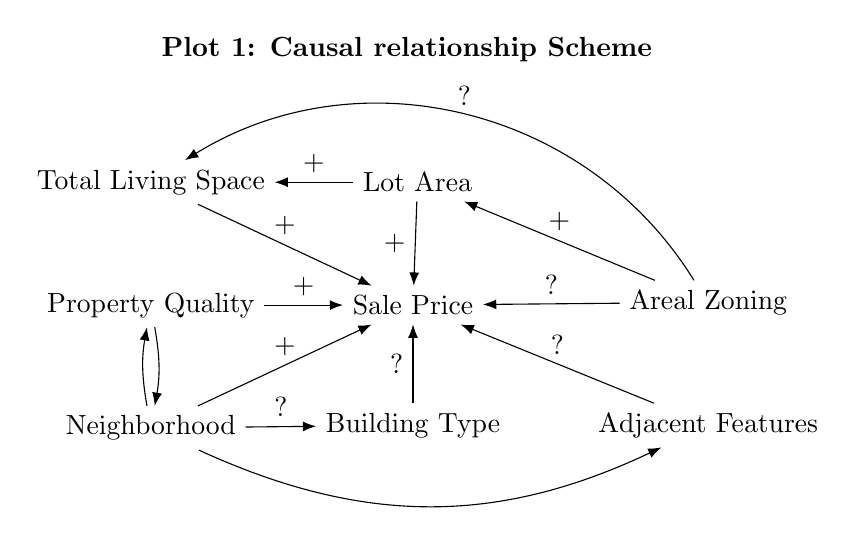
\begin{tikzpicture}
	\centering
 	\node at (3.25,3.25) {\textbf{Plot 1: Causal relationship Scheme}};
    \node (1) at (0,0) {Property Quality};
	\node (2) [above = of 1] {Total Living Space};
	\node (3) [right = of 1] {Sale Price};
	\node (4) [below = of 3] {Building Type};
	\node (5) [right = of 4] {Adjacent Features};
	\node (6) [above = of 5] {Areal Zoning};
	\node (7) [below = of 1] {Neighborhood};
	\node (8) [right = of 2] {Lot Area};
	
	\path (7) edge node[above] {$+$} (3);
	% \path (7) edge node[left] {$?$} (2);
	\path (7) edge[bend left=10](1);
	\path (1) edge[bend left=10](7);
	\path (8) edge node[above] {$+$}(2);
	\path (2) edge node[above] {$+$}(3);
	\path (1) edge node[above] {$+$}(3);
	\path (8) edge node[left] {$+$}(3);
	\path (4) edge node[left] {$?$}(3);
	\path (7) edge node[above] {$?$}(4);
	\path (6) edge node[above] {$+$}(8);
	\path (7) edge[bend right=25](5);
	\path (5) edge node[above] {$?$}(3);
	\path (6) edge node[above] {$?$}(3);
	\path (6) edge[bend right=45] node[above] {$?$}(2);

\end{tikzpicture}
\end{center}











\indent The first category of data pertains to the size dimension of the house in
question. Here the size of the house (1stFlrSF + 2ndFlrSF), combined with
further information regarding the of bathrooms (BsmtFullBath + FullBath),
Bedrooms (Bedroom), and Kitchen explain the overall living space of a house
or appartment. Additionally, the lot size (LotArea) of the property and the
garage (GarageCars/GarageArea) specification complement this category.

The Second category describes neighborhood and location related characteristics of the property. School districts (indirectly included as unobservable!!!) and afluent neighborhoods naturally have a large impact on the saleprice. Additionally, neighborhoods may, thus, function as cluster correction for similarities in the error term when correcting for heteroscedasticity; assuming that sales in the same neighborhood share similar underlying variation. Finally, the neighborhood may control for the size of the house; we would generally assume that big houses are more expensive. However, if we consider New York downtown, to large houses in the country side of Iowa, small flats (in new york) might induce that small properties cost more than large properties. 

The third category of data distinguishes in the type of housing that was recorded as a sale in the data (MSSubClass, BldgType). 

The fourth category focuses on the quality and condition aspect of the property as a function of years since remodeling (YearRemodAdd), building finalize date (YearBuilt), and the overall rating of quality (OverallQual) and condition (OverallCond) of the property.





Note, variables such as central heating have been discarded as those usually are contained in the type of house (appartments tend to have central administered heating from the overall building).

MAKE A CAUSAL SCHEME!!!! HErE IN LATEX








\end{document}